\let\negmedspace\undefined
\let\negthickspace\undefined
\documentclass[journal]{IEEEtran}
\usepackage[a5paper, margin=10mm, onecolumn]{geometry}
%\usepackage{lmodern} % Ensure lmodern is loaded for pdflatex
\usepackage{tfrupee} % Include tfrupee package

\setlength{\headheight}{1cm} % Set the height of the header box
\setlength{\headsep}{0mm}     % Set the distance between the header box and the top of the text

\usepackage{gvv-book}
\usepackage{gvv}
\usepackage{cite}
\usepackage{amsmath,amssymb,amsfonts,amsthm}
\usepackage{algorithmic}
\usepackage{graphicx}
\usepackage{textcomp}
\usepackage{xcolor}
\usepackage{txfonts}
\usepackage{listings}
\usepackage{enumitem}
\usepackage{mathtools}
\usepackage{gensymb}
\usepackage{comment}
\usepackage[breaklinks=true]{hyperref}
\usepackage{tkz-euclide} 
\usepackage{listings}
% \usepackage{gvv}                                        
\def\inputGnumericTable{}                                 
\usepackage[latin1]{inputenc}                                
\usepackage{color}                                            
\usepackage{array}                                            
\usepackage{longtable}                                       
\usepackage{calc}                                             
\usepackage{multirow}                                         
\usepackage{hhline}                                           
\usepackage{ifthen}                                           
\usepackage{lscape}
\usepackage{circuitikz}
\tikzstyle{block} = [rectangle, draw, fill=blue!20, 
    text width=4em, text centered, rounded corners, minimum height=3em]
\tikzstyle{sum} = [draw, fill=blue!10, circle, minimum size=1cm, node distance=1.5cm]
\tikzstyle{input} = [coordinate]
\tikzstyle{output} = [coordinate]


\begin{document}

\bibliographystyle{IEEEtran}
\vspace{3cm}

\title{4.8.13}
\author{AI25BTECH11017-BALU}
 \maketitle
% \newpage
% \bigskip
{\let\newpage\relax\maketitle}
\renewcommand{\thefigure}{\theenumi}
\renewcommand{\thetable}{\theenumi}
\setlength{\intextsep}{10pt} % Space between text and floats
\numberwithin{equation}{enumi}
\numberwithin{figure}{enumi}
\renewcommand{\thetable}{\theenumi}
\textbf{Question}:\\
 Find the distance between the planes 
\begin{align}
\vec{r} \cdot (2\hat{i} - 3\hat{j} + 6\hat{k}) - 4 = 0
\quad \text{and} \quad
\vec{r} \cdot (6\hat{i} - 9\hat{j} + 18\hat{k}) + 30 = 0.
\end{align}
.\\
\solution \\
Let us solve the given equation theoretically and then verify the solution computationally \\
According to the question, \\
Given two planes with direction vectors\\
\begin{align}
\vec{n_1}=\begin{myvec}{2\\-3\\6}\end{myvec}\
\vec{n_2}=\begin{myvec}{6\\-9\\18}\end{myvec}\
\end{align}
\begin{align}
    \vec{n_2}=3\vec{n_1}
\end{align}
so the are planes are parllel\\
Let us take a point in plane 1
\begin{align}
    \vec{A}=\begin{myvec}{2\\0\\0}\end{myvec}
\end{align}
As planes are parllel distance from $\vec{A}$ to plane 2 is same as distance between planes\\
Let distance is k\\
\begin{align}
    k=\frac{(\vec{A}\vec{n_2}^T)+30}{\|\vec{n_2}\|}=2
\end{align}
\begin{figure}[h!]
    \centering
    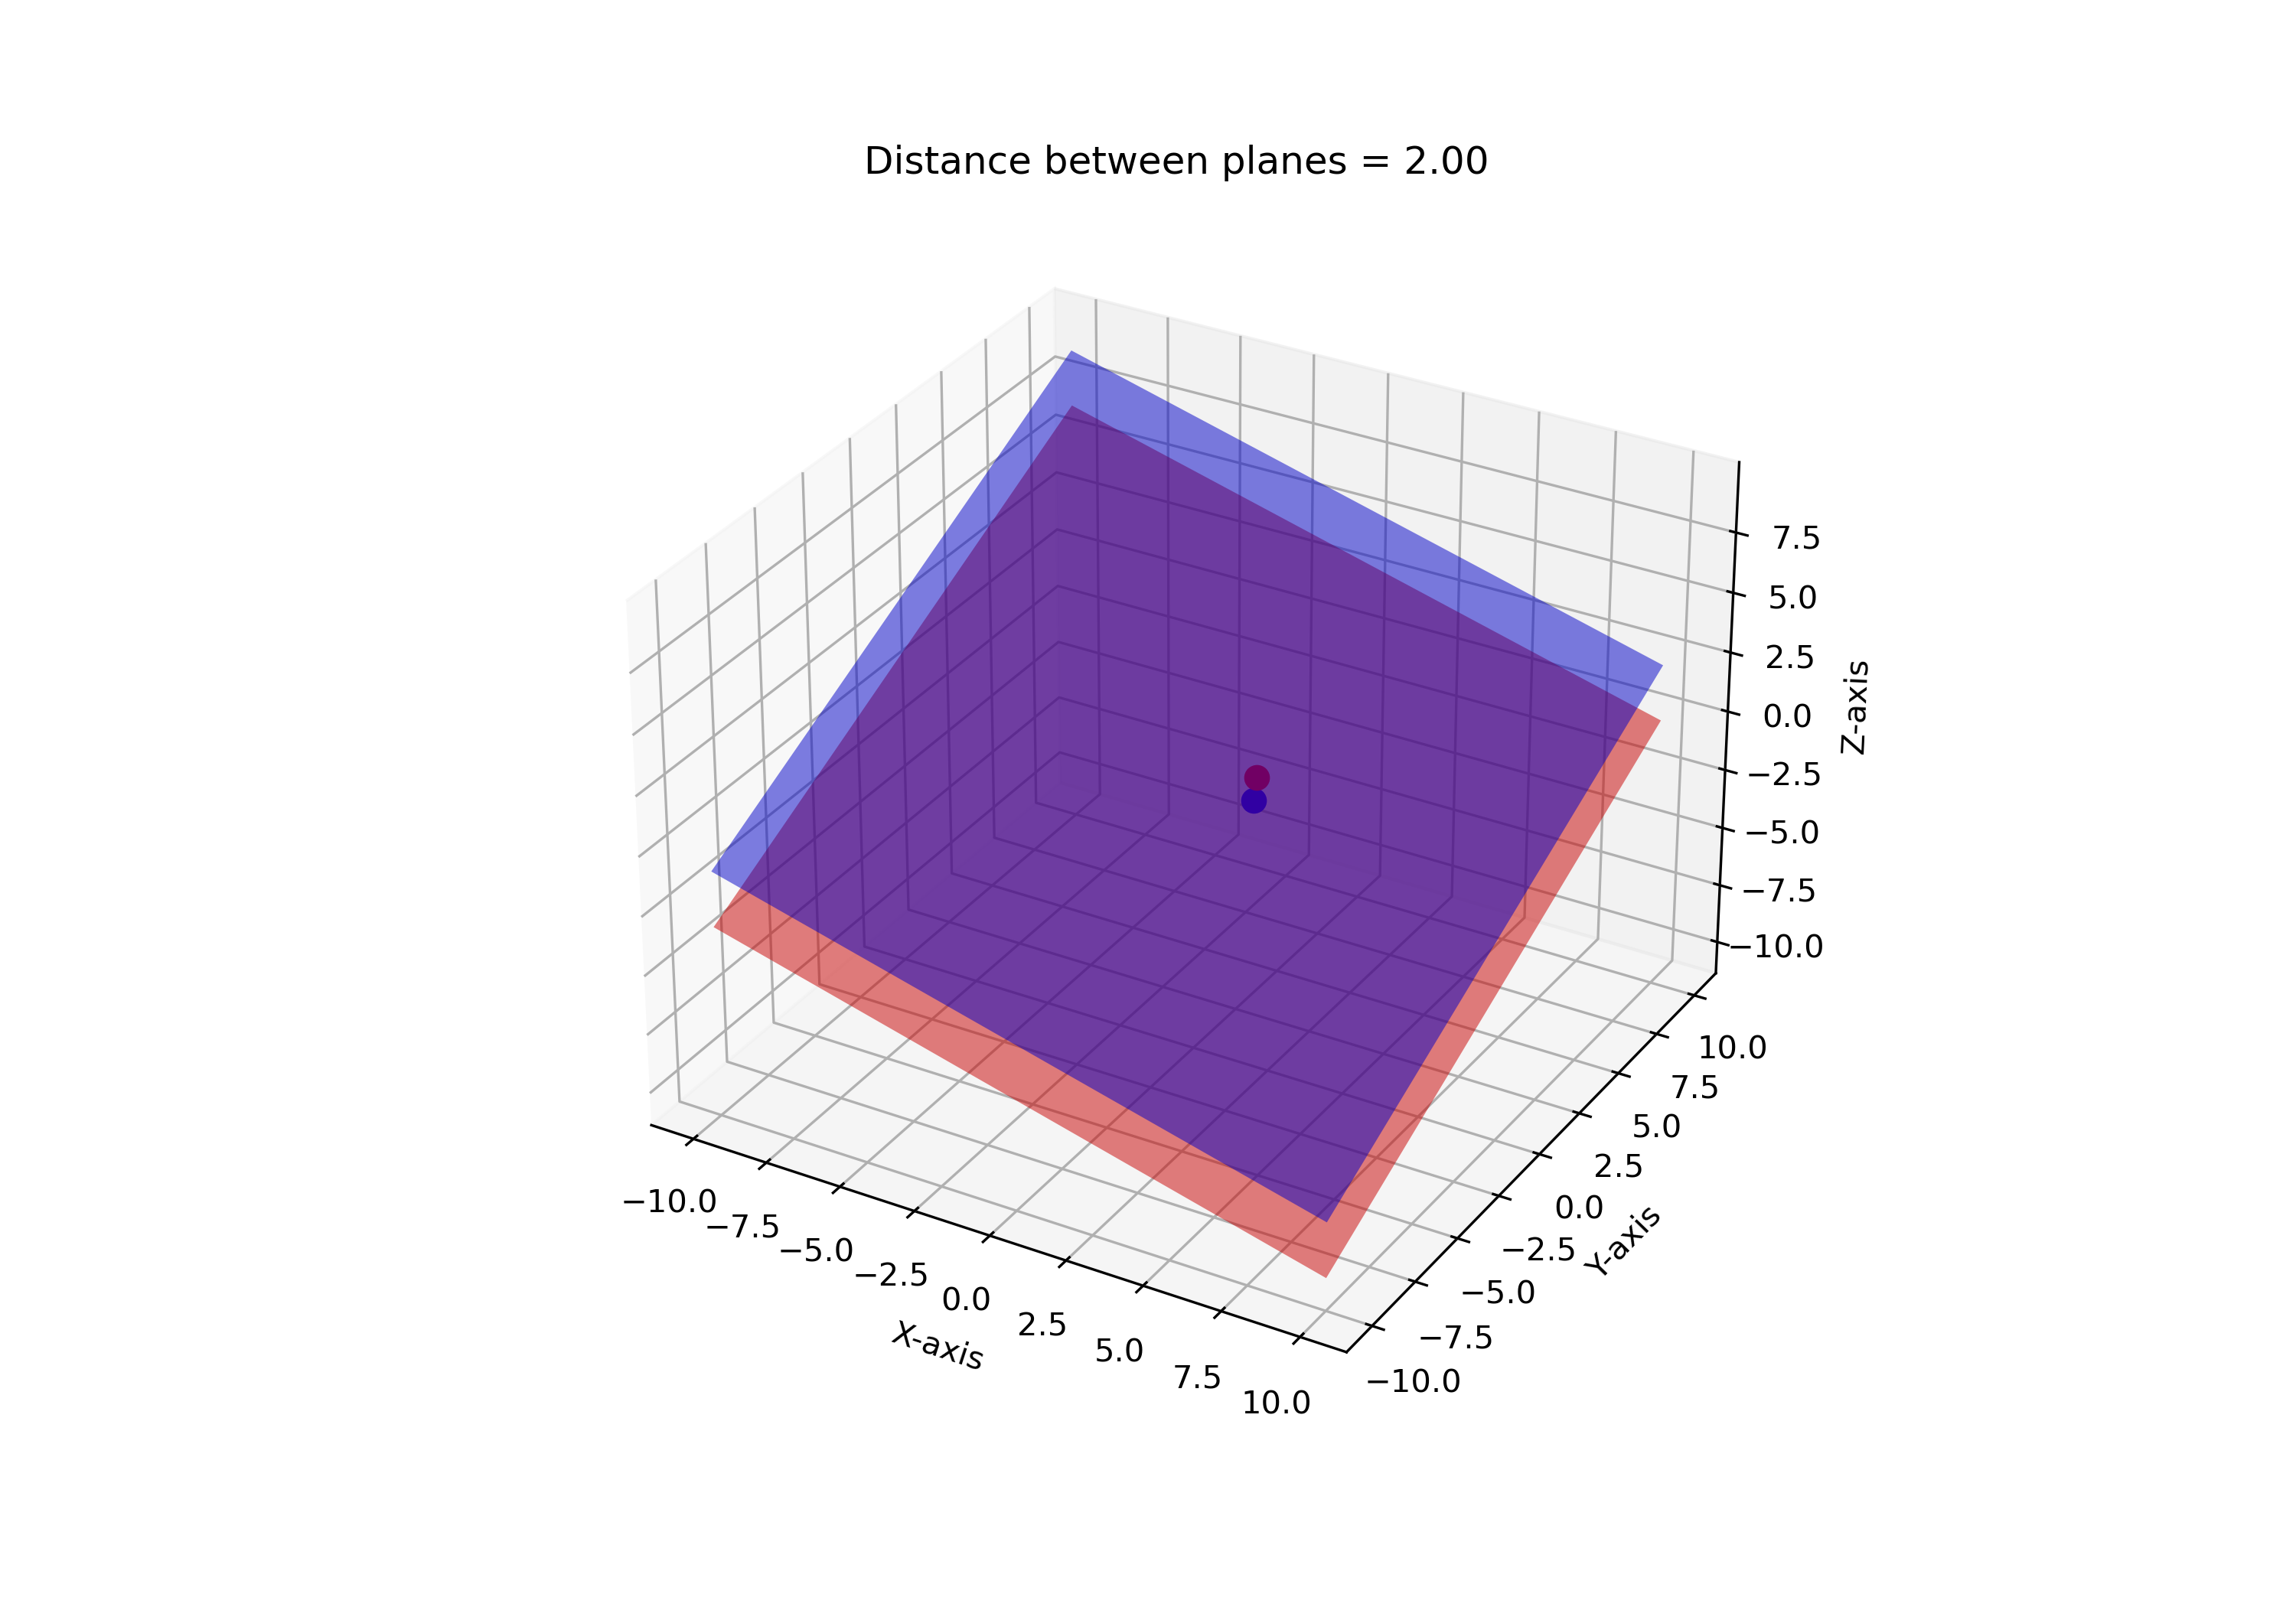
\includegraphics[width=0.8\columnwidth]{figs/planes_distance.png}
    \caption{}
    \label{fig:placeholder}
\end{figure}
\end{document}